\subsection{Positionsbestimmung}
UND FUNKTIONSWEISE


In diesem Kapitel wird zunächst einmal geklärt, was Positionsbestimmung ist. 
Nach Alex Küpper ist die Positionsbestimmung wie folgt definiert:

\begin{table}[h]
	\centering
	\begin{tabular}{|p{16cm}|}\hline
		\textbf{Zitat ?:} \glqq Positioning is a process to obtain the spatial position of a target \grqq  \cite[S.121]{Kuepper2005} \\ \hline
		\textbf{Übersetzung:} Positionsbestimmung ist ein Prozess, um die räumliche Position eines Ziels zu erhalten. \\ \hline
	\end{tabular}
\end{table}

Mit räumlicher Position ist hierbei ein Standort gemeint, der zu einem geeigneten Bezugssystem bestimmt wird. Das bedeutet ein Position der sich auf das Bezugssystem „Weltkarte“ bezieht repräsentiert den geografischen Standort auf der Weltkarte. Die Position mit dem Bezugssystem eines bestimmten Gebäudes repräsentiert den Standort in dem Gebäude. Bsp.: Stockwerk 1 Raum 139b.

Ein weiteres Zitat bezüglich der Positionsbestimmung grenzt den Begriff Positionsbestimmung deutlich von Ortung ab. Dieser Unterschied soll hier auch aufgezeigt werden. Hierzu das Zitat der Webseite www.itwissen.info:

\begin{table}[h]
	\centering
	\begin{tabular}{|p{16cm}|}\hline
		\textbf{Zitat ?:} \glqq Die Begriffe Positionsbestimmung und Ortung werden häufig synonym benutzt; sie unterscheiden sich allerdings im Detail. So wird mit der Positionsbestimmung der Ort von Objekten oder Personen eindeutig in einem geografischen Koordinatensystem festgelegt. Sie bildet die Basis für die Ortung und wird dann zur Ortung, wenn Dritten die ermittelte Position mitgeteilt wird. \grqq  \cite[Positionsbestimmung]{itwissen} \\ \hline
	\end{tabular}
\end{table}

Das Zitat ist aussagekräftig und grenz Positionsbestimmung und Ortung eindeutig voneinander ab.

In diesem Kapitel wird, wie es der Titel vorgibt, nur die Positionsbestimmung betrachtet. Dieser ist die Voraussetzung, um Ortung (die Übertragung der Position) überhaupt durchzuführen. Allerdings wird im weiteren Teil dieser Arbeit verstärkt die Ortung betrachtet werden. Die Übertragung der Position spielt nämlich zur Bereitstellung eines „location based Services“ in nahezu allen Fällen eine große Rolle. Da die Positionsbestimmung für die Ortung benötigt wird, diese hier im Detail vorgestellt.

TODO: Küpper S.123
Fundamentals ergänzen??

Bei einer Positionsbestimmung werden Messdaten gesammelt, um die eigenen Position festzulegen. Die Messdaten beziehen sich dabei immer auf festgelegte Fixpunkte, von welchen die Position schon bekannt ist.  Diese Daten sind zum Beispiel Winkel, Geschwindigkeit und Entfernung.

In den kommenden Kapiteln werden unterschiedliche Methoden/Techniken zur Positionsbestimmung aufgezeigt. Diese werden in drei Kategorien eingeordnet, die satellitengestützte Positionierung, Positionierung in Mobilfunknetzen und Positionsbestimmung in Gebäuden.

TODO: Robustheit ergänzen???

Kein Verfahren zur Positionsbestimmung ist perfekt. 
Deshalb werden die unterschiedlichen Methoden/Techniken zur Positionsbestimmung anhand von drei ?Qualitäts?-Merkmalen betrachtet. Diese werden hier kurz erläutert.

\begin{enumerate}
\item Bereich (Scope)\\
Ein Positionssystem ist immer auf einen Bereich bezogen, in dem eine Position theoretisch bestimmt werden kann. Dieser Bereich kann stark variieren von einem Raum bis zu einem weltweiten Bereich.\\
--> Ein großer Scope ist besser
\item Abdeckung (Coverage)\\
Die Abdeckung eines Positionssystems kann maximal so groß sein, wie es der Bereich zulässt. Die Abdeckung ist die Teilmenge des Bereichs, in dem tatsächlich die Position bestimmt werden kann. So ist es beispielsweise bei einem Satellitenpositionssystem nicht möglich eine Abdeckung in Gebäuden oder unter der Erde zu gewährleisten.\\
--> Eine große Abdeckung ist besser
\item Präzision (Precision)\\
Ein Positionssystem kann einen Standort nicht exakt, sondern mit einer gewissen Abweichung bestimmen. Diese Abweichung kann von Umwelteinflüssen abhängen und für eine Positionsbestimmung an der selben Stelle abweichende Ergebnisse liefern. Die Robustheit eines Positionssystem trägt somit zur Präzision bei. \\
-->Eine höhere Präzision ist besser
\end{enumerate}
\cite[S.183]{Schiller2004}


\textbf{Satellitengestützte Positionierung}

Satellitengestützte Positionierung basiert, wie der Name schon vermuten lässt, auf Satelliten. 

Das bekannteste System zur satellitengestützte Positionierung ist das Global Positioning System, dass mit GPS abgekürzt wird. Auf GPS wird nach einer Erläuterung über das generelle Funktionsprinzip von Satellitenpositionierung eingegangen.

Gegeben für eine Positionsbestimmung sind Satelliten, die sich in der Erdumlaufbahn befinden und elektromagnetische Wellen auf die Erde funken. Damit eine Position auf der Erdoberfläche mit Hilfe von Satelliten errechnet/bestimmt werden kann, muss zuerst einmal ein Gerät vorhanden sein, dass die elektromagnetischen Wellen der Satelliten empfangen kann.

Ist das gegeben kann prinzipiell die Position des Nutzers auf der Erdoberfläche anhand von der exakten Position von mindestens drei Satelliten ($s_{n}$) und des Abstands zu diesen Satelliten ($r_{m}$) bestimmt werden.

\cite[S. 188]{Schiller2004}

Vergleiche hierzu Abbildung \ref{fig:Grundprinzip Satelliten}

\begin{figure}[h]
\centering
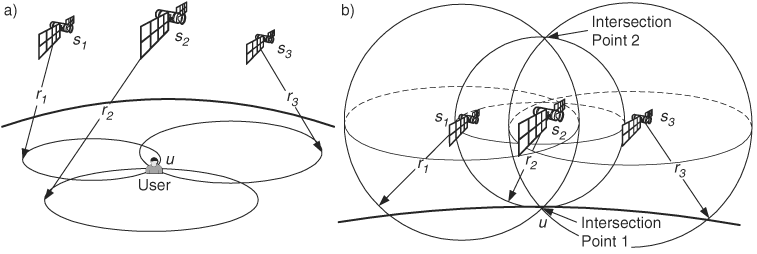
\includegraphics[width=0.99\textwidth]{ref/images/prinzip_satelliten.png}
\caption[Grundprinzip Satelliten Positionsbestimmung]{Grundprinzip Satelliten Positionsbestimmung}
\label{fig:Grundprinzip Satelliten}
\cite[S. 188]{Schiller2004}
\end{figure}

In Abbildung \ref{fig:Grundprinzip Satelliten} a) stellen die Kreise Positionen auf der Erde dar, an denen ein User-Position anhand des gemessenen Abstands ($r_{m}$) möglich ist. In dieser Darstellung mit drei Satelliten ist die User-Position eindeutig an dem Schnittpunkt aller drei Kreise. In Abbildung \ref{fig:Grundprinzip Satelliten} b) wird die Darstellung ins dreidimensionale überführt. Hierbei ist nun zu erkennen, dass die Kreise zu Kugeln geworden sind. Daraus resultierend gibt es nun einen zweiten Schnittpunkt. Für die Positionsbestimmung gibt es nun zwei mögliche User-Positionen. Dieses Problem beseitigt man einfach, indem man die logisch wahrscheinlichere Position als richtige ansieht. In der Abbildung wäre das Intersection Point 1, da Intersection Point 2 im Weltall liegt und davon auszugehen ist, dass sich Menschen auf der Erdoberfläche befinden.

Es wurde nun erläutert, wie sich die Position ermitteln lässt, wenn dem Nutzer die Position der Satelliten und der Abstand zu diesen bekannt ist. Wie diese Werte ermittelt werden wurde noch nicht erwähnt. Darauf wird nun eingegangen.

Satelliten Positionen:\\
%ref/images/GPS_Umlaufbahn.PNG S.164 Küpper
Bild + Erklärung fixe Umlaufbahnen. Die Positionen können aus Daten über Satellitenname und Umlaufbahn errechnet werden. Diese Daten werden mit einem GPS gerät ausgeliefert und bei Bedarf (Ausfall eines Satelliten oder neuer Satellit aktualisiert)

Abstand zu den Satelliten:\\
Der Abstand zu Satelliten wird anhand von der Zeit berechnet, die das Signal vom Satelliten bis zum Empfänger benötigt. Diese Zeit wird dadurch ermittelt, dass ein vom Satelliten die aktuelle Zeit gesendet wird. Sobald diese beim Empfänger ankommt wird der Zeitunterschied $ \bigtriangleup t $ zur aktuellen Zeit ermittelt. Da sich elektromagnetische Wellen mit Lichtgeschwindigkeit $ c $ fortbewegen, beträgt die Geschwindigkeit näherungsweise 300.000 $km/s$. Mit der Formel $ r = c \bigtriangleup t$ lässt sich dann die Entfernung zum Satelliten ermitteln. Das Verfahren funktioniert allerdings nur, wenn die Uhren vom Satelliten und des Empfängers exakt synchronisiert sind. 

Verfahren zur Uhren Synchronisation:\\
Eine Abweichung der Uhren von nur $1\mu s$ ergibt aufgrund der hohen Geschwindigkeit der elektromagnetischen Wellen eine Abweichung der bestimmten Position von ca. 300 Metern. \cite[S. 189]{Schiller2004}


--> Bereich (Scope) prinzipiell ist eine Standortbestimmung auf der ganzen Welt möglich

--> Abdeckung (Coverage) Die Position kann überall auf der Erdoberfläche, mit einer Ausnahme, der Positionsbestimmung in Gebäuden, bestimmt werden. Das bietet eine sehr große Abdeckung

--> Präzision (Precision) eine hohe Präzision wird durch vielen Satelliten und Korrektursignale ermöglicht. Die Position ist recht robust gegen Umwelteinflüsse, wie Wolken oder 

\cite{Schiller2004}

\underline{GPS}



\textbf{Positionierung in Mobilfunknetzen}


\textbf{Positionsbestimmung in Gebäuden}



\textbf{GPS, Mobilfunk, WLAN, Bluetooth}

\subsubsection{Kriterien für die Standortbestimmung}
Genauigkeit, Bestimmungszeit, Robustheit


\subsubsection{Arten der Standortbestimmung}
GPS, Mobilfunk, WLAN, Sterne, Beacons